% Please do not change the document class
\documentclass{scrartcl}

% Please do not change these packages
\usepackage[hidelinks]{hyperref}
\usepackage[none]{hyphenat}
\usepackage{setspace}
\doublespace

% You may add additional packages here
\usepackage{amsmath}
\usepackage{graphicx}

% Please include a clear, concise, and descriptive title
\title{Is it ethical for game designers to make their games addictive-like?}

% Please do not change the subtitle
\subtitle{COMP230 - Ethics and Professionalism}

% Please put your student number in the author field
\author{1702208}

\begin{document}

\maketitle

\section{Introduction}

Nowadays video games have become a very common way of spending time among adolescents and adults. Although playing games have both negative and positive effects. Positive effects are usually stress reduction\cite{russoniello2009effectiveness}, relaxation\cite{wack2009relationships}, emotional disturbances in children\cite{jones2014gaming}\cite{hull2009computer} and a lot more. But there are still some negative consequences. Besides the most common - addiction - there are aggression, antisocial behaviour and violence, that usually depends on the game itself. But in this paper, main focus will be set on addiction, which still requires further learning. 

\section{Video game ethics}

\section{Skinner box}

Some games are intentionally designed to be addictive. That way they are putting players into a digital Skinner box. So-called Skinner box, also called an operant conditioning chamber \cite{skinnerbox}, was developed by Burrhus Frederic Skinner - ``American psychologist and an influential exponent of behaviourism"\cite{bfskinner}. He was studying human behaviour ``in terms of responses to environmental stimuli"\cite{bfskinner}. His Skinner box metaphor is related to players being addictive to a certain game whether they want that or not\cite{creepyaddiction}. 

This experiment was based on a laboratory rat, or other small animal, being put in a small glass box equipped with drinking tubes, food pellets and a bar or key that can be pressed\cite{skinnerbox}\cite{nyskinnerbox}\cite{creepyaddiction}. First, it was given a food pellet by looking at the lever, after - getting close to it and, eventually, pressing the lever. But not every press would give a food pellet, which made the rat press the lever continuously to sometimes get its reward\cite{nyskinnerbox}. Moreover, some presses could dispense an unpleasant reinforce. For example, lights, sounds or images or, in the worst case, the floor may be electrified\cite{skinnerbox}.

\subsection{}
When Skinner was running out of food pellets for his experimental rat, he started giving one for every ten pressed instead of one\cite{behavioralgd}. Thus, he discover a new area of psychology, that is often used for game design\cite{behavioralgd}. Ratios and intervals appeared as a sort of contingencies. This makes players to keep "pressing that lever" to get rewards. If a player knew he would get something every time he does that he would relax and not worry about not getting rewards\cite{creepyaddiction}. But giving random number of presses to get that reward makes player's rapidly and continuously "press the lever". Therefore, keeping them playing the game for much longer.

This experiment relates to human behaviour as well. This is very well shown in games when designers intend to reward player for their continuous efforts, but rewards are not always satisfying for players or there are no reward at all. This stimulates them to play more and more to eventually get that reward and therefore get closer to achieving one's personal goal.

\section{Player's fault or developers' intentions?}

Addictive games are usually most of the Massive Multi-player Online Role Playing Games (MMORPGs), Competitive games and casual/mobile games. Casual games are designed to give us satisfaction for a minimal input\cite{vgaddiction}. Whereas MMORPGs and competitive games stimulate us to play more and more of these games by levelling up or constantly getting better at the game. It generates previously mentioned digital Skinner box. Players are always looking for a rewards and therefore continuing to play this game in hope of getting better gear and levelling up. This is shown in picture \ref{fig:comic} in a comic way. Nevertheless, it's very accurate about most MMORPGs.

\begin{figure}
  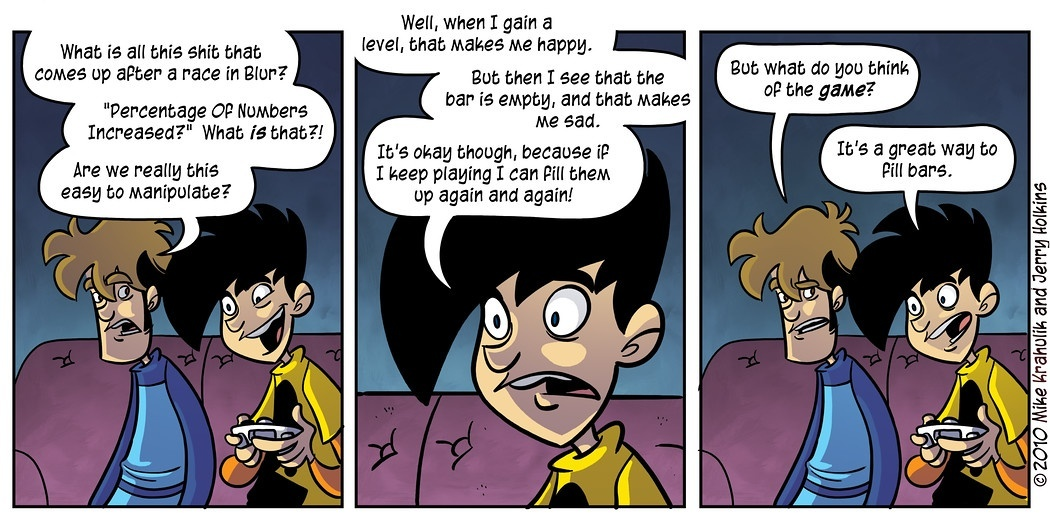
\includegraphics[width=\linewidth]{Images/AddictionComic.jpg}
  \caption{Addiction comic.}
  \label{fig:comic}
\end{figure}

\subsection{Level grinding for rewards}
Competitive games are hooking due to their skill-based gameplay. The more you play the better you get. And therefore, the more enjoyable and challenging it is to play with and against players with the same skill level. But there are games where it also includes levelling system. An example is League of Legends, made by Riot Games. It's a MOBA game with levelling system and about a year ago they deleted level cap, which was thirty. For every level player gets a small reward - a loot box - which can be opened for free, but gives only in-game currency for purchasing characters and a character component, character of which can be purchased for lower price. In addition to that, they removed opportunity to receive that in-game currency by playing games, which made players grind for levels to get that currency and buy their wanted character.

\subsection{Why is Free-to-Play addictive?}
Free-to-play games can also be addictive by being designed to ``monetize the seven deadly sins"\cite{vgaddiction}. This means having:

\begin{itemize}
	\item \textbf{Lust} - wanting that in-game item;
	\item \textbf{Gluttony} - getting that in-game consumable;
	\item \textbf{Avarice} - having everything in the game;
	\item \textbf{Sloth} - speeding up grinding;
	\item \textbf{Wrath} - getting a revenge on a player;
	\item \textbf{Envy} - having better gear than others;
	\item \textbf{Pride} - looking cooler than others.
\end{itemize}
And everything must be paid real life money for that. This also includes previously mentioned game. 

\section{Conclusion}

It is certainly unethical to make players continuously play their game for years and, often enough, even invest money for in-game loot. This makes addiction even worse as it adds a gambling element, which is addictive by itself. But there are cases where players are looking for an addictive-like game, where they have to grind for levels and items. In this case, they want to have an "offline" relaxation method, that does not include real life problems and responsibilities. As video game designer Erin Hoffman said: ``Addiction is not about what you do, but what you don't do because of the replacement of the addictive behavior"\cite{addictivegamemechs}.

\bibliographystyle{ieeetran}
\bibliography{references}

\end{document}
